\documentclass[11pt,a4paper]{article}

\usepackage[a4paper,top=2.4cm,bottom=2.4cm,left=2.2cm,right=2.2cm]{geometry}
\usepackage{fontspec}
\usepackage[spanish,provide=*]{babel}
\babelprovide[import]{spanish}
\babelprovide[import]{english}
\babelfont{rm}{Noto Serif}
\babelfont{sf}{Noto Sans}
\babelfont{tt}{Noto Sans Mono}
\usepackage{amsmath,amssymb}
\usepackage{booktabs}
\usepackage{enumitem}
\usepackage{xcolor}
\usepackage{tikz}
\usetikzlibrary{arrows.meta,positioning,shapes.geometric,fit,backgrounds}
\usepackage[colorlinks=true,linkcolor=blue!60!black,citecolor=blue!60!black,urlcolor=blue!60!black]{hyperref}
\setlist[itemize]{label=--,leftmargin=*}
\setlist[enumerate]{leftmargin=*}
\emergencystretch=2em

\title{\textbf{ASTRA Production}\\[2mm]
\large Arquitectura autónoma de razonamiento y validación de teoremas científicos}
\author{Nelson Bolívar\\\textit{Science-Stack Research Group}}
\date{Versión de arquitectura: septiembre de 2026}

\begin{document}
\maketitle

\begin{abstract}
ASTRA Production (\textit{Autonomous Symbolic Theorem Reasoning Architecture}) es un motor multiagente de investigación que transforma una intuición científica en una hipótesis falsable, la traduce a un experimento computacional ejecutable y somete el resultado a análisis crítico antes de aceptar una conclusión. Su principio central es separar la generación lingüística de la evidencia: los modelos de lenguaje proponen, formalizan y analizan; un oráculo de cálculo simbólico o numérico ejecuta el programa de validación y devuelve evidencia reproducible. El sistema admite ciclos aislados y campañas autónomas de investigación, varios proveedores de modelos, motores matemáticos locales o remotos, corrección automática de código, aprobación humana de teoremas e informes persistentes. Un segundo principio de diseño gobierna qué ocurre cuando un ciclo no puede concluir. En lugar de forzar un veredicto o agotar su presupuesto repitiéndose, ASTRA detecta que un bucle de revisión dejó de avanzar, declara un estado explícito de indecidibilidad cuando al validador le faltan entradas, y devuelve una petición estructurada de los valores ausentes en vez de un fallo silencioso. Este documento describe la arquitectura implementada actualmente, sus garantías, sus límites y el estado presente de su evaluación.
\end{abstract}

\section{Motivación y principio epistemológico}

Los modelos de lenguaje son útiles para formular hipótesis, conectar dominios y escribir programas, pero una respuesta plausible no constituye una demostración. ASTRA adopta por ello una división explícita de responsabilidades:

\begin{itemize}
  \item la \textbf{capa heurística} propone conjeturas, genera código y explica resultados;
  \item la \textbf{capa de ejecución} calcula con motores simbólicos, numéricos o lógicos reales;
  \item la \textbf{capa de control} conserva el estado, aplica reintentos, protege el veredicto y solicita decisiones humanas;
  \item la \textbf{capa documental} registra código, salida, análisis, proveedores y evolución de la investigación.
\end{itemize}

La afirmación de trabajo no es que ASTRA automatice la verdad matemática, sino que convierte el razonamiento asistido por IA en un proceso inspeccionable:
\[
\begin{aligned}
\text{intuición}&\longrightarrow\text{hipótesis falsable}
\longrightarrow\text{programa}\\
&\longrightarrow\text{evidencia ejecutada}
\longrightarrow\text{veredicto revisable}.
\end{aligned}
\]

La salida de un modelo nunca reemplaza la ejecución. A su vez, una ejecución exitosa no basta por sí sola: el programa debe representar correctamente la afirmación y producir una señal discriminante entre validación y refutación.

\section{Arquitectura vigente}

ASTRA se ejecuta como una aplicación local con interfaz web. El servidor Flask expone la interfaz y una API de control; un orquestador asíncrono mantiene la máquina de estados en segundo plano. Los agentes se comunican con proveedores LLM mediante una capa común, mientras que el oráculo enruta el código hacia el motor adecuado. La interfaz web, el servidor MCP y la herramienta por subproceso invocan el mismo ciclo canónico: no mantienen implementaciones científicas paralelas.

\begin{figure}[htbp]
\centering
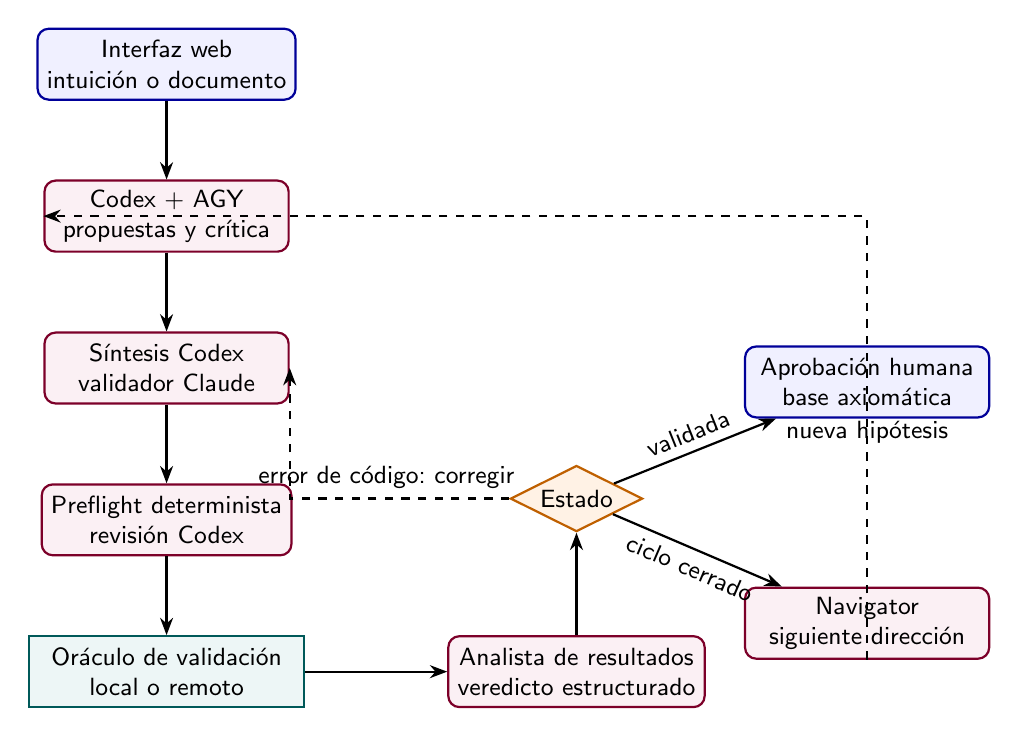
\begin{tikzpicture}[
  node distance=10mm and 9mm,
  font=\sffamily\small,
  ui/.style={rectangle,rounded corners,draw=blue!60!black,fill=blue!6,thick,align=center,minimum width=31mm,minimum height=9mm},
  agent/.style={rectangle,rounded corners,draw=purple!65!black,fill=purple!6,thick,align=center,minimum width=31mm,minimum height=9mm},
  oracle/.style={rectangle,draw=teal!70!black,fill=teal!7,thick,align=center,minimum width=35mm,minimum height=9mm},
  gate/.style={diamond,aspect=2,draw=orange!75!black,fill=orange!10,thick,align=center,inner sep=1.5pt},
  arr/.style={-{Stealth[length=2.2mm]},thick}
]
\node[ui] (input) {Interfaz web\\intuición o documento};
\node[agent,below=of input] (conj) {Codex + AGY\\propuestas y crítica};
\node[agent,below=of conj] (trans) {Síntesis Codex\\validador Claude};
\node[agent,below=of trans] (review) {Preflight determinista\\revisión Codex};
\node[oracle,below=of review] (exec) {Oráculo de validación\\local o remoto};
\node[agent,right=18mm of exec] (analyst) {Analista de resultados\\veredicto estructurado};
\node[gate,above=13mm of analyst] (status) {Estado};
\node[ui,above right=8mm and 17mm of status] (human) {Aprobación humana\\base axiomática};
\node[agent,below right=9mm and 17mm of status] (nav) {Navigator\\siguiente dirección};

\draw[arr] (input)--(conj);
\draw[arr] (conj)--(trans);
\draw[arr] (trans)--(review);
\draw[arr] (review)--(exec);
\draw[arr] (exec)--(analyst);
\draw[arr] (analyst)--(status);
\draw[arr] (status)--node[above,sloped]{validada}(human);
\draw[arr] (status)--node[below,sloped]{ciclo cerrado}(nav);
\draw[arr,dashed] (status.west) -| node[pos=.28,above]{error de código: corregir} (trans.east);
\draw[arr,dashed] (nav.south) |- node[pos=.28,below]{nueva hipótesis} (conj.west);
\end{tikzpicture}
\caption{Flujo lógico de ASTRA Production. El Navigator interviene en el modo de investigación; la aprobación humana protege la incorporación de resultados a la base axiomática.}
\label{fig:architecture}
\end{figure}

\subsection{Entrada e interfaz}

El usuario puede introducir una afirmación directamente o cargar material PDF/TXT. La aplicación ofrece dos modalidades:

\begin{itemize}
  \item \textbf{Ciclo único}: evalúa una intuición concreta mediante una pasada completa.
  \item \textbf{Bucle de investigación}: descompone una pregunta macroscópica en una secuencia de conjeturas relacionadas y mantiene ramas alternativas.
\end{itemize}

La interfaz muestra el estado, la conjetura vigente, el script generado, la salida del oráculo, la base axiomática, los informes y el registro de eventos. También permite detener la ejecución, aprobar o rechazar resultados y configurar los proveedores por rol. La caché de ciclos incluye el objetivo, la base axiomática, el resumen de la trayectoria reflexiva, la distancia al último hito y la configuración no secreta de modelos y controles; por ello una dirección repetida en un contexto científico nuevo no reutiliza una navegación obsoleta.

\subsection{Estructuración de la petición}

Una petición cruda suele arrastrar varias afirmaciones a la vez, o enuncia un propósito sin criterio decidible. Una etapa opcional previa al ciclo la reescribe como afirmación acotada, hipótesis explícita, prueba decisiva con sus verificaciones auxiliares, ruta propuesta, entradas que esa prueba necesita y lo que se difiere a propósito. El ciclo trabaja entonces sobre la forma estructurada mientras el texto original se conserva junto a ella, de modo que el lector siempre puede ver qué se pidió y qué se probó. La etapa es opcional porque cuesta una llamada de modelo y una petición bien planteada no la necesita.

Su valor práctico está en la lista de entradas. Una petición que nombra las cantidades que el validador va a necesitar puede responderse antes de arrancar el ciclo, lo que sale más barato que descubrir el hueco después de formalizar.

\subsection{Agente de conjeturas}

Codex GPT-5.6 Sol y AGY reciben el mismo objetivo final, la dirección actual y el contexto acumulado. Proponen en paralelo, cada uno critica adversarialmente la propuesta rival y Codex sintetiza una única conjetura falsable con variables, supuestos, dominio y criterio de éxito. En el modo iterativo también utilizan teoremas establecidos y refutaciones anteriores para evitar repetir rutas cerradas.

\subsection{Traductor formal}

El traductor convierte la conjetura en un script autocontenido. El código debe calcular una cantidad verificable: un residual simbólico, una identidad, condiciones iniciales, una desigualdad, un contraejemplo, una propiedad tensorial o una comparación numérica con tolerancias explícitas. Puede declarar el motor mediante una cabecera como \texttt{ASTRA\_ENGINE} y sugerir ejecución local o remota con \texttt{ASTRA\_ORACLE}.

El traductor no emite el veredicto científico. Construye el experimento que permitirá decidirlo.

\subsection{Preflight y revisión independiente}

Antes de ejecutar, controles deterministas buscan patrones que podrían producir una validación falsa, errores de importación y fallos operacionales conocidos. Codex compara luego el script de Claude con el objetivo compartido y la conjetura exacta. Si encuentra un defecto reparable, Claude recibe instrucciones acotadas y devuelve un parche de reemplazos exactos. Codex no pasa a ser autor del validador. Un rechazo del revisor o un parche no aplicable produce abstención o error de herramienta, nunca evidencia científica.

El bucle está acotado por dos vías independientes. Un tope de revisiones limita cuántas veces puede parcharse o regenerarse el validador, y un control de reloj detiene un bucle que consumiría el presupuesto del ciclo solo en reparar. Ninguna de las dos diagnostica por qué falla el bucle, así que hay un tercer mecanismo. Cada rechazo se clasifica por el defecto que describe, leyendo la prosa del revisor y no su lista de instrucciones, porque esas instrucciones enumeran las patas que hay que conservar y por eso se parecen en todas las rondas. El clasificador reconoce un conjunto pequeño de defectos recurrentes, entre ellos una cota supuesta, una positividad indecidible, un vínculo afirmado solo en un comentario, un sustituto en lugar de la cantidad de interés, un dominio sin restringir y un muestreo presentado como demostración.

La respuesta escala con la evidencia. Un defecto visto una vez produce una corrección dirigida que lo nombra. La misma clase vista de nuevo se toma como señal de que parchear no va a converger, y el ciclo gasta una regeneración en una estrategia distinta en lugar de otro parche. Si la clase sobrevive también a eso, el ciclo se detiene limpiamente e informa de la clase de defecto que no pudo despejar. Una parada así es una abstención con causa nombrada, que es más útil que un presupuesto agotado en silencio. El detector está activo por defecto y puede desactivarse para comparaciones controladas.

\subsection{Oráculo de validación}

El oráculo ejecuta el programa y captura código de retorno, salida estándar, errores y metadatos del motor. Python constituye la base común, con bibliotecas como SymPy, Z3, NumPy, SciPy, mpmath, EinsteinPy, Pint, fluids y QuTiP. ASTRA también puede enrutar trabajos a SageMath, Maxima o Cadabra cuando están disponibles. En Windows, \texttt{ASTRA\_WSL\_DISTRO} fija la distribución WSL2 deseada para que la ejecución no cambie silenciosamente si se modifica la distribución predeterminada de la máquina. La estación de producción utiliza Debian/WSL2 para SageMath, Maxima, Cadabra y el entorno local Lean/Mathlib.

La ejecución puede ser:

\begin{itemize}
  \item \textbf{local}, adecuada para álgebra simbólica y cálculos moderados;
  \item \textbf{remota}, mediante un trabajador Linux por SSH para cargas pesadas, GPU o herramientas instaladas en la estación de cálculo.
\end{itemize}

La política puede fijarse por configuración o inferirse de marcadores y características del script. La ausencia de un motor opcional debe producir un fallo explícito, no una validación ficticia.

\subsection{Analista y guardia de veredicto}

El analista recibe la conjetura y la evidencia bruta. Devuelve una respuesta estructurada con uno de estos estados:

\begin{center}
\begin{tabular}{@{}ll@{}}
\toprule
Estado & Significado \\
\midrule
\texttt{VALIDATED} & La evidencia computacional respalda la hipótesis formulada. \\
\texttt{REFUTED} & La ejecución produce un contraejemplo o contradice la hipótesis. \\
\texttt{NON\_DECIDABLE} & La prueba no puede instanciarse porque faltan entradas declaradas. \\
\texttt{CODE\_ERROR} & El programa no logró ejecutar correctamente la prueba. \\
\texttt{API\_ERROR} & Falló el proveedor LLM, la red o la cuota correspondiente. \\
\bottomrule
\end{tabular}
\end{center}

Un sexto estado, \texttt{WEAK\_PASS}, no lo produce el analista sino que se le impone. La guardia de veredicto audita el árbol sintáctico del validador y degrada un aprobado que ninguna rama de fallo alcanzable podría haber contradicho, que es la firma de una prueba incapaz de fallar. Cuando análisis independientes discrepan, gana la lectura más prudente bajo una precedencia fija, con la refutación por delante de la indecidibilidad, esta por delante del error de código y cualquiera de ellas por delante de la validación. El fallo de proveedor se trata aparte, porque no contiene ningún contenido científico.

Cuando aparece \texttt{CODE\_ERROR}, ASTRA solicita código corregido y repite la validación hasta el límite configurado. La guardia de veredicto restringe conclusiones incompatibles con la evidencia de ejecución. Esto reduce, aunque no elimina, el riesgo de que el analista convierta un fallo técnico en una afirmación científica.

\subsection{Cuando faltan las entradas}

Un validador que no puede instanciarse no es una refutación ni un error de programación, y sin embargo durante casi toda la historia de ASTRA se registró como lo segundo. Una prueba a la que le faltaba un valor de frontera, una constante material o un ansatz no llegaba a correr, se clasificaba como error de código y consumía el presupuesto entero de reparación regenerando un programa que nunca fue el problema.

El estado indecidible convierte ese caso en ciudadano de primera. Lo declara el propio validador, imprimiendo un marcador de veredicto seguido de una línea por cada entrada ausente y saliendo con un código reservado. La declaración tiene que venir del validador. El analista solo puede confirmar un resultado indecidible cuando el programa declaró uno, de modo que el estado no puede inventarse después para excusar un fallo. Se permite un reintento si el analista insiste en que el programa sencillamente estaba roto. Una segunda declaración, o una reparación que el autor reporta como imposible, cierra el ciclo.

\subsection{Preguntar en vez de detenerse}

Terminar sin decidir es un desenlace honesto pero un mal valor por defecto, porque el dato que falta suele tenerlo el investigador. ASTRA no dispone de un canal propio hacia el usuario, así que la pregunta viaja en el resultado hacia el agente que invocó el ciclo. Un resultado indecidible lleva una petición que nombra las entradas ausentes y tres maneras de responderla, cada una con la reinvocación exacta que la implementa. El usuario puede aportar los valores, puede ordenar al ciclo que suponga valores declarados y continúe, o puede hacer que el agente los extraiga de un fichero o de un resultado anterior.

La suposición está deliberadamente acotada. Un validador que corre bajo esa política debe declarar cada valor supuesto en su propia línea, esas declaraciones quedan adheridas al resultado como condiciones, y una corrida que supuso algo nunca puede certificar el objetivo completo. Su cobertura permanece parcial y su estado permanece atómico. A un validador al que se le concedió la política de suposición y no declaró nada se lo trata como si hubiera supuesto en silencio, que es el caso más peligroso, y se lo marca igual. Las respuestas reutilizan la conjetura ya pagada a través del punto de control del propio ciclo, de modo que contestar a la pregunta reanuda en el validador y no en el principio.

\subsection{Aprobación humana y base axiomática}

Una hipótesis marcada como validada queda en espera. Sólo después de la aprobación del investigador se incorpora como teorema establecido. Las refutaciones, con su justificación, también alimentan el contexto para bloquear caminos ya descartados. Esta puerta humana reconoce que la corrección del programa, los supuestos físicos y el alcance de la conclusión todavía requieren juicio experto.

\section{Bucle autónomo de investigación}

En una campaña, ASTRA mantiene una \textit{Research Session} asociada a una pregunta macroscópica. Después de cada ciclo, el Navigator evalúa el progreso y propone:

\begin{itemize}
  \item la siguiente dirección en profundidad;
  \item ramas paralelas que conviene conservar;
  \item si se alcanzó un hito que requiere revisión;
  \item si la pregunta macroscópica puede considerarse resuelta.
\end{itemize}

Si una conjetura fue validada, el sistema puede generalizarla, explorar sus fronteras o aplicarla a otro régimen. Si fue refutada, busca una alternativa que evite la causa concreta del fracaso. El investigador puede continuar con la propuesta, redirigir el trabajo o activar una rama guardada. En modo autónomo, ASTRA atraviesa los hitos sin pausa hasta que el Navigator declara resolución, se alcanza el tiempo máximo o el usuario detiene la sesión.

Este procedimiento es profundidad-primero con memoria de ramas; no equivale a una búsqueda exhaustiva ni garantiza que la declaración de resolución sea correcta.

\section{Control de ASTRA desde un agente}

ASTRA no está limitado a su interfaz web. El servidor \textit{Model Context Protocol} (MCP) expone el oráculo como herramientas que pueden invocar Codex, Claude Code, Gemini u otro cliente compatible. De este modo, el agente que conversa con el investigador puede formular el plan, escribir el programa de prueba, pedir la ejecución y examinar la evidencia sin copiar manualmente resultados entre aplicaciones.

La interfaz ha crecido hasta unas veinte operaciones agrupadas en seis familias:

\begin{center}
\small
\begin{tabular}{@{}lp{10.0cm}@{}}
\toprule
Familia & Operaciones \\
\midrule
Deliberación & \texttt{astra\_cycle} ejecuta conjetura, traducción, revisión, oráculo y análisis en una pasada. \texttt{astra\_cycle\_submit} hace lo mismo desacoplado, para ciclos más largos que el muro de herramienta del cliente. \\
Ejecución & \texttt{astra\_execute} corre un script ya escrito en el oráculo local, remoto o automático. \\
Trabajos & \texttt{astra\_submit} y \texttt{astra\_job} lanzan y sondean cálculo desacoplado con salida incremental. \\
Observación & \texttt{astra\_probe} lee la fase y el \textit{heartbeat} de un ciclo vivo sin interrumpirlo. \texttt{astra\_telemetry} resume el conjunto de ciclos terminados. \texttt{astra\_status}, \texttt{astra\_engines} y \texttt{astra\_capacity} informan de la alcanzabilidad del trabajador, los motores disponibles y las plazas libres de ciclo. \\
Campañas & \texttt{astra\_campaign\_*} arrancan, avanzan, inspeccionan, pausan y reanudan un programa de varios ciclos. \\
Clúster & \texttt{astra\_cluster\_*} envían, sondean y cancelan trabajo en la estación de cómputo. \\
\bottomrule
\end{tabular}
\end{center}

Un ciclo invocado por esta interfaz acepta los mismos campos de petición que exponen la estructuración y la maquinaria de entradas descritas arriba, que es lo que permite a un agente responder a un resultado indecidible sin reconstruir la llamada original.

El MCP se registra apuntando el cliente al intérprete del entorno de ASTRA y a \path{mcp_server/server.py}; después se abre una sesión nueva del agente para cargar las herramientas. El investigador puede entonces pedir, por ejemplo: ``formula una prueba independiente del escalar de Ricci, ejecútala con \texttt{astra\_execute} y no aceptes el resultado hasta revisar los residuales''. Para cálculos de más de unos minutos conviene usar \texttt{astra\_submit} y seguirlos con \texttt{astra\_job}.

Esta modalidad convierte al agente conversacional en la capa de planificación y a ASTRA en la capa de ejecución trazable. El agente no recibe autoridad adicional: sigue obligado a presentar código, supuestos, salida y criterio de decisión.

\section{Extensión mediante motores y paquetes científicos}

La capa del oráculo es extensible y no constituye una lista cerrada. Todo paquete disponible en el entorno donde corre el script puede participar en una validación. Entre los paquetes científicos desarrollados por el propio equipo se encuentran:

\begin{center}
\path{GR_python}\quad \path{pyWarpFactory}\quad \path{warp_bubble_optimization}.
\end{center}

El requisito de integración es sencillo: el script debe poder importar el paquete, fijar entradas reproducibles, producir evidencia inspeccionable y terminar con un veredicto explícito. El mismo paquete debe instalarse en el entorno local o en el trabajador remoto elegido.

Esta capacidad permite reutilizar solvers, métricas, optimizadores, análisis de condiciones de energía y bancos de pruebas ya validados. Para disminuir errores comunes, una conclusión importante debería combinar patas independientes: por ejemplo, una identidad simbólica, evaluaciones numéricas con semilla fija y un límite conocido.

\subsection{Lean 4 y Mathlib}

Lean 4 se integra como motor opcional mediante la marca \texttt{\# ASTRA\_ENGINE: lean}. El traductor puede generar un archivo que importe Mathlib; ASTRA lo entrega a un proyecto nativo fijado, al proyecto fijado en Debian/WSL2 o a la ruta formal configurada en ASTRUM. La ruta local de producción fija Lean 4.30.0 y el commit de Mathlib que comienza por \texttt{c5ea00351c28}. La aceptación por el kernel de Lean proporciona verificación mecánica apropiada para lógica formal, matemáticas discretas, álgebra y teoremas que ya puedan expresarse en el lenguaje del asistente de pruebas.

Lean no sustituye los cálculos físicos numéricos ni prueba que la formalización represente correctamente al sistema real. Su garantía se aplica al enunciado formal y a los axiomas importados. Si el compilador rechaza la prueba, ASTRA lo clasifica como error de código y puede solicitar una corrección; nunca debe convertir el rechazo en una refutación del teorema.

\subsection{Wolfram Mathematica como oráculo complementario}

Cuando el modelo dispone del complemento de Wolfram o de Mathematica Agent Bridge, el agente puede escribir y ejecutar Wolfram Language directamente. El bridge local comunica procesos externos con un kernel de Mathematica mediante una cola JSON y puede operar sobre un notebook abierto o en modo \textit{headless} con \texttt{wolframscript}. Entre sus acciones se encuentran:

\begin{center}
\path{evaluate-wl}, \path{simplify-symbolic}, \path{compare-expressions},
\path{commutator} y \path{gr-curvature}.
\end{center}

El bridge también permite leer, escribir y evaluar celdas.

Mathematica puede actuar como segundo validador independiente: el agente ejecuta una prueba en ASTRA y repite la identidad, el tensor o el límite con el bridge. La concordancia entre motores de implementación distinta fortalece la evidencia; una discrepancia obliga a revisar convenciones, dominios y supuestos. El bridge evalúa código con los privilegios del usuario local, por lo que sólo debe habilitarse para agentes y carpetas de comandos confiables.

\section{Proveedores, motores y despliegue}

Los roles pueden reasignarse para estudios de ablación, pero el contrato de producción compacto es explícito: Codex CLI con \texttt{gpt-5.6-sol} y esfuerzo \texttt{xhigh} propone, sintetiza, revisa y analiza; AGY con \texttt{gemini-3.1-pro-high} y esfuerzo \texttt{high} co-propone, critica y navega como nivel primario, con \texttt{gemini-3.7-flash-high} como primer respaldo configurado y \texttt{gemini-3.5-flash-high} como respaldo legado; Claude Code con \texttt{claude-opus-4-8} escribe y repara el código. La orden \texttt{scripts/audit\_architecture.py} verifica este mapa, los binarios, las puertas epistémicas, los motores científicos locales y las rutas formales sin leer ni imprimir secretos. \texttt{ASTRA\_REQUIRED\_LOCAL\_ENGINES} convierte la ausencia de un motor de producción en un fallo bloqueante de auditoría. El script idempotente \path{scripts/bootstrap_wsl_scientific_stack.ps1} reconstruye la pila Debian fijada. Otros proveedores compatibles se reservan para comparaciones controladas.

A los proveedores se llega por sus clientes de línea de comandos de suscripción y no por API medida, así que la restricción operativa es una ventana de uso por modelo y no un precio por token. Cada rol lleva por eso una escalera ordenada de modelos. Un fallo de cuota baja la escalera y el resultado registra qué peldaño respondió, mientras que un fallo de calidad la sube, promoviendo al autor a un modelo más fuerte exactamente cuando la guardia determinista ha demostrado que el más barato no bastaba. La prueba de un proveedor adicional corre por la misma capa de cliente dentro de WSL y se trata como un rol configurable más.

La configuración que podría cambiar un resultado científico queda estampada en cada ciclo. El manifiesto de arquitectura registra el mapa de roles, los modelos efectivos, las puertas epistémicas y los motores locales exigidos, y participa en la clave de caché del ciclo junto a una versión de esquema. Cambiar un control invalida por tanto los ciclos cacheados en lugar de reutilizar en silencio resultados producidos bajo otras reglas.

La instalación de escritorio crea un entorno Python y arranca la interfaz en \url{http://127.0.0.1:5050}. Las credenciales y parámetros del oráculo se mantienen en configuración local y no deben incorporarse al repositorio. ASTRA conserva sesiones e informes en el espacio de trabajo de la aplicación.

\section{Persistencia, trazabilidad y calibración}

Cada ciclo genera informes HTML y Markdown con la intuición, conjetura, script, resultado de ejecución, análisis y proveedores utilizados. Las investigaciones pueden guardarse, recargarse y revisarse desde el historial. La suite de \textit{benchmarks} incluye problemas de relatividad general, ecuaciones diferenciales, fluidos, lógica, sistemas cuánticos y cálculo simbólico.

Los \textit{benchmarks} cumplen dos funciones: comprobar que los motores siguen operativos y comparar la capacidad de distintos proveedores para construir pruebas discriminantes. No sustituyen la validación científica del problema nuevo, pero detectan regresiones de infraestructura y sesgos sistemáticos.

\section{Observabilidad e higiene de ejecución}

Un ciclo que tarda veinte minutos es normal, y durante casi toda la historia de ASTRA fue además opaco. Tres mecanismos hacen ahora que una corrida sea inspeccionable mientras ocurre y auditable después.

Cada ciclo escribe un latido que nombra su fase actual, el tiempo consumido por cada fase completada y el punto de control al que pertenece. Un proceso lector puede así informar del avance sin tocar el ciclo. En Windows cada ciclo abre además su propia consola con la instrucción, la fase, la ronda de revisión, una barra de progreso y una estimación de finalización calculada con las medianas de los ciclos terminados recientes. La ventana se lanza mediante un trampolín desacoplado para que matar un ciclo vencido no destruya también el único relato de lo que estaba haciendo. Una observabilidad que muere con el proceso que observa vale poco justo cuando hace falta.

Las corridas de prueba se mantienen fuera del registro de producción. Los conjuntos que lee la telemetría son los puntos de control terminados y los latidos vivos, y una suite que ejercita ciclos reales escribía en ambos, lo que distorsionaba toda duración media y todo recuento de desenlaces. Una variable de raíz de espacio de trabajo redirige los artefactos del ciclo, y la sesión de pruebas la apunta a un directorio temporal. Sin la variable las rutas son byte a byte las de siempre, de modo que el comportamiento de producción no cambia.

También se espera que el sistema falle de forma inteligible en contextos hostiles. Cuando se conduce ASTRA desde una sesión aislada cuyo testigo de acceso no puede escribir en su propio espacio de trabajo, la fase se detiene ahora de inmediato con un error explícito de permisos que nombra el directorio y las dos salidas posibles. Antes se colgaba, porque la plataforma declara un directorio escribible atendiendo solo a su lista de acceso y sin consultar un testigo restringido, y la rutina estándar de temporales se fía de esa declaración y reintenta. Por la misma razón la auditoría de instalación distingue un motor ausente de un motor simplemente inalcanzable desde el contexto actual, ya que decirle a alguien que reinstale una herramienta que funciona es peor que no decirle nada.

\section{Garantías y límites}

ASTRA mejora la reproducibilidad porque conserva y ejecuta el programa, pero no convierte automáticamente una prueba computacional en una demostración universal. Persisten varias obligaciones:

\begin{itemize}
  \item verificar que la conjetura formal corresponde a la pregunta original;
  \item inspeccionar que el código no compruebe una versión debilitada o circular;
  \item distinguir evidencia numérica, identidad simbólica y demostración lógica;
  \item declarar dominios, unidades, condiciones de frontera y tolerancias;
  \item repetir resultados sensibles a precisión, malla o plataforma;
  \item someter las conclusiones relevantes a revisión humana independiente.
\end{itemize}

Los estados añadidos desde julio traen sus propias salvedades, y son más estrechos de lo que sugiere su nombre:

\begin{itemize}
  \item \texttt{NON\_DECIDABLE} registra que este validador, tal como está escrito, no pudo instanciarse con las entradas disponibles. Es una afirmación sobre un programa y un conjunto de entradas, nunca sobre que la pregunta sea indecidible en principio.
  \item Un veredicto producido bajo la política de suposición queda condicionado a valores que eligió el modelo. Es evidencia sobre una familia parametrizada, y los valores supuestos deben leerse junto con él.
  \item Una parada atribuida a una clase de defecto repetida acota el coste. No establece que la objeción del revisor fuera correcta, solo que parchear dejó de converger.
  \item El clasificador de defectos lee prosa escrita por un modelo y puede equivocarse. Es una heurística para repartir el presupuesto restante, no parte de la cadena de evidencia.
\end{itemize}

Por ello, \texttt{VALIDATED} significa ``validado por el oráculo bajo el programa y los supuestos registrados'', no ``verdad matemática absoluta''. La fortaleza de ASTRA reside en hacer visible y repetible la cadena de evidencia.

\section{Estado de la evaluación}

Este documento describe una arquitectura. Todavía no reporta una ventaja medida, y la distinción importa lo suficiente como para enunciarla sin rodeos.

Lo ejecutado es un conjunto de pilotos de integración, un caso por corpus externo, corridos el 24 de julio de 2026 contra SciCode, un problema de olimpiada de FrontierScience, un ítem de validación de miniF2F y una tarea de repositorio de AInsteinBench. Establecen que la tubería corre de extremo a extremo sobre material público y que el revisor y el bucle de reparación se comportan según diseño en esos casos. No son resultados de tabla comparativa, los informes crudos se conservan fuera del control de versiones y ninguna afirmación de rendimiento comparado se apoya en ellos.

Una comparación defendible exige el split oficial completo de cada benchmark, prompts y presupuestos fijos, reintentos declarados, versiones de evaluador registradas, fallos contados en el denominador, intervalos de confianza y la métrica nativa de cada corpus, reportado con tiempo de pared y número de llamadas de modelo.

La medición que pondría a prueba esta arquitectura de forma más directa es más estrecha que todo eso y es el próximo experimento previsto. La afirmación central de diseño es que separar al autor de un validador de su revisor, entre proveedores de modelo distintos, atrapa defectos que un solo modelo revisando su propio trabajo no atrapa. Esa afirmación se somete a prueba por ablación a presupuesto igual, comparando la configuración de producción contra una en la que el modelo autor también revisa, y contra otra sin revisión independiente alguna, midiendo cuántos validadores defectuosos llegan al oráculo en cada brazo. Hasta que ese experimento se corra y sus registros queden depositados, el argumento a favor de la arquitectura aquí presentada es de construcción y trazabilidad, no de exactitud demostrada.

\section{Conclusión}

ASTRA Production ha evolucionado desde un esquema de procesamiento fijo hacia una arquitectura de investigación multiagente, configurable e iterativa. La formulación, la traducción, la ejecución, el análisis, la navegación y la aprobación son responsabilidades diferenciadas. El trabajo desde julio ha tratado menos de añadir capacidad que de acotar el fallo, para que un ciclo incapaz de concluir diga qué entrada le falta, qué defecto no pudo despejar o qué permiso se le negó, en vez de consumir su presupuesto en silencio. El oráculo aporta una referencia externa al discurso de los modelos; los informes preservan la trazabilidad; y la puerta humana impide que la autonomía se confunda con autoridad científica. El resultado es una plataforma para investigar con modelos de lenguaje sin delegarles silenciosamente el criterio final de verdad.

\end{document}
